\documentclass[UTF8]{ctexart}
\usepackage{subfigure}
\usepackage{caption}
\usepackage{amsmath,bm}
\usepackage{amssymb}
\usepackage{pifont}
\usepackage{geometry}
\usepackage{graphicx}
\usepackage{gensymb}
\usepackage{wrapfig}
\usepackage{titlesec}
\usepackage{float}
\usepackage{diagbox}
\usepackage{fancyhdr}
\usepackage{color}
\usepackage{bm}
\usepackage{siunitx}
\usepackage{ulem}
\usepackage{CJKulem}
\pagestyle{plain}
\geometry{a4paper,scale=0.8}
\CTEXsetup[format+={\raggedright}]{section} 
\title{固物2020期末}
\author{Deschain}
\titlespacing*{\section}
{0pt}{0pt}{0pt}
\titlespacing*{\subsection}
{0pt}{0pt}{0pt}
\titlespacing*{\paragraph}
{0pt}{0pt}{0pt}
\titlespacing*{\subparagraph}
{0pt}{0pt}{0pt}
\titleformat*{\section}{\normalsize}
\begin{document}
\maketitle
\section*{1.填空题(每空1分,共45分)}
(1)具有长程有序的固体结构,即原子按照一定的周期规律排列的固体物质,称为\uline{{\color{white} 晶体}},为了描述这种周期性结构,
将这种空间排列称为\uline{{\color{white} 晶格}},周期性重复单元称为\uline{{\color{white} 晶胞}},其中体积最小的称为
\uline{{\color{white} 原胞}}。\\
(2)Si的晶体结构为\uline{{\color{white} 面心立方}}结构,Si原子之间以\uline{{\color{white} 共价}}键结合,属于\uline{{\color
{white} 复式}}(简单/复式)晶格,其对应的布拉菲格子为\uline{{\color{white} 面心立方}}格子,倒格子为\uline{{\color{white} 体心立方}}
格子。布里渊区为在倒格子空间中,以某倒格点为中心,由中心格点到相邻格点的连线的垂直平分线所围成的多面体。\\
(3)单晶硅在常温下\uline{{\color{white} 能}}导电,离子晶体在低温下\uline{{\color{white} 不能}}导电。(能/不能)\\
(4)有效质量与电子质量可以有很大差别,这是由于有效质量包含了\uline{{\color{white} 晶格的周期性势场}}的作用。能带顶部的电子的有效质量为
\uline{{\color{white} 负}},此时在外场作用下,电子从外场获得的动量\uline{{\color{white} 小于}}(大于/小于)它交给晶体的动量。\\
(5)一般情况下,本征半导体的费米能级$E_{F_i}$可以近似认为位于\uline{{\color{white} 带隙中央}}。N型掺杂半导体的费米能级
$E_{F_n}$向\uline{{\color{white} 导带}}靠近;P型掺杂半导体的费米能级$E_{F_P}$向\uline{{\color{white} 价带}}靠近(导带/价带)。若P型
掺杂浓度为$N_a$,温度为$T$,则有关系式$E_{F_i}-E_{F_P}=k_BTln(\frac{N_a}{n_i})$。\\
(6)一般半导体材料中电子的迁移率\uline{{\color{white} >}}($>/</=$)空穴迁移率,这主要是由于\uline{{\color{white} 空穴}}的有效质量
更大。\\
(7)经典电子论中,电子的功函数为电子真空能级与\uline{{\color{white} 导带底}}的能量差,由材料本身的性质决定;而量子理论中电子的功函数为
电子真空能级与\uline{{\color{white} 费米能级}}的能量差。\\
(8)有一掺杂半导体,当温度从0K开始逐渐升高至其熔点时,半导体中的载流子浓度会经历先\uline{{\color{white} 增大}},然后\uline{{\color
{white} 基本不变}},最后再\uline{{\color{white} 增大}}的过程。\\
(9)PN结的形成。在P型半导体和N型半导体结合后,在其交界处产生了电子和空穴的浓度差,故电子会从N区向P区发生\uline{{\color{white} 扩散}}
运动。该运动的结果使得交界面出P区一侧失去\uline{{\color{white} 空穴}}留下带\uline{{\color{white} 负}}电的杂质离子,N区同理。这些不能
移动的带电粒子在交界面附近形成了\uline{{\color{white} 空间电荷区}},其中的电场方向为\uline{{\color{white} 从N区指向P区}},电场强度在
\uline{{\color{white} 空间电荷区中间某位置}} ,其宽度与掺杂浓度成\uline{{\color{white} 反比}}。另一方面,该电场使P区和N区的
\uline{{\color{white} 少数}}(多数/少数)载流子向另一侧发生\uline{{\color{white} 漂移}}运动。最后,这两种运动达到动态平衡。\\
(10)一般的PN结在正常导通工作时,正极应接在\uline{{\color{white} P}}(P/N)区。光电二极管也是由一个PN结组成的器件,当有特定频率的光入
射到结区时,结区会产生大量电子——空穴对,若想将光生载流子引出形成光电流,还需要外加偏压,此时正极应接在\uline{{\color{white} N}}(P/N)区。\\
(11)如果要使金属和N型半导体形成肖特基接触,需要金属功函数\uline{{\color{white} >}}($>/</=$)半导体功函数,肖特基势垒高度等于金属功函数
和半导体\uline{{\color{white} 电子亲和能}}之差。\\
(12)简单晶格中的格波不存在\uline{{\color{white} 光学波}}(声学波/光学波);复式晶格的固体中格波存在光学波和声学波。从物理意义的角度看,
长波极限时,复式晶格声学波的特征为原胞做整体运动,频率较\uline{{\color{white} 低}}(高/低);而光学波的特征为\uline{{\color{white} 
相邻原子位相相反,同种原子位相相同}},频率较\uline{{\color{white} 高}}。\\
(13)某一维原子链中有$N$个原子,相邻原子间距为$a$。考虑周期性边界条件,若为单原子链,则简约布里渊区$(-\frac{\pi}{a},\frac{\pi}{a})$中
格波波数的取值总数为\uline{{\color{white} N}}。若为交替排列的双原子链,简约布里渊区中格波波数的取值总数为\uline{{\color{white} 2N}}。\\
(14)霍尔效应的实际应用。如图1所示,某沿y,z方向厚度皆为1cm的长方体未知掺杂半导体材料,沿+x方向通50mA的稳恒电流,沿z方向加磁感应强度为0.5T
的静磁场,得到y=0cm和y=0.1cm面间的电势差为+0.4mV。则该材料为\uline{{\color{white} P}}型掺杂,载流子浓度为\uline{{\color{white} 
$3.90625\times10^{21}m^{-3}$}}。(洛伦兹力遵循左手定则)\\
\begin{figure}[H]                                        
    \centering                                                
    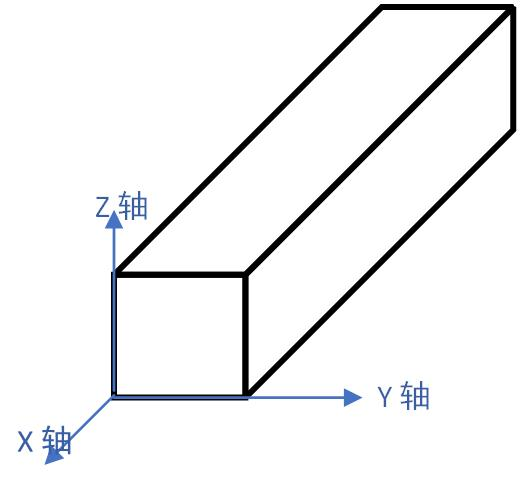
\includegraphics[width=4cm,height=4cm]{图1.jpg}        
    \caption{}                                                                                  
\end{figure}                                              
\section*{2.(12分)石墨烯是一种C原子按正六边形排列的二维晶体,如图2所示,图中黑点代表C原子。相邻两个C原子间距为0.142nm(本题中长度相关
单位量纲请用nm,数值计算误差在5\%以上视为错误。)}
\begin{figure}[H]                                        
    \centering                                                
    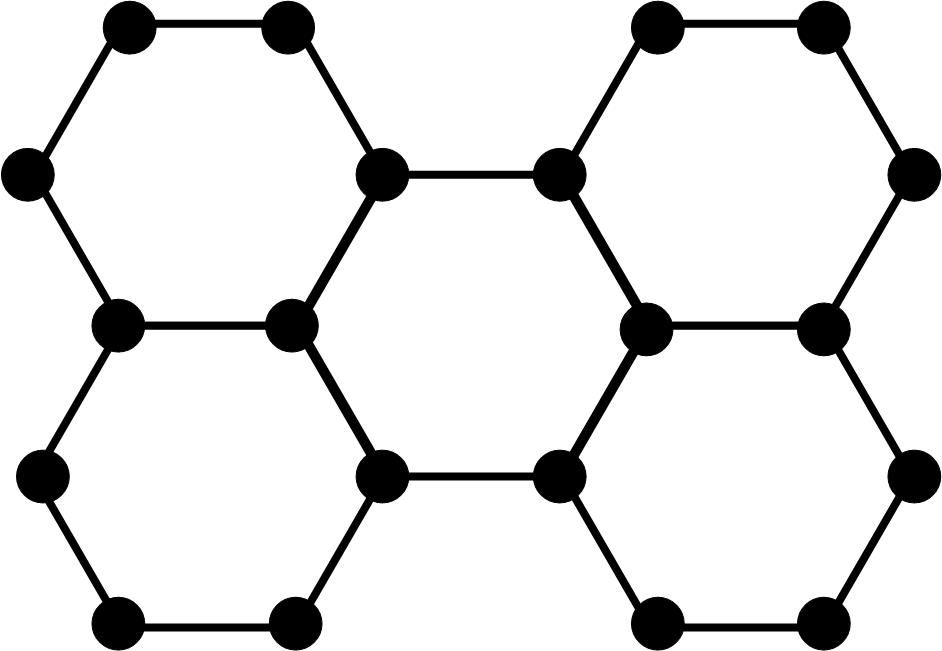
\includegraphics[width=6cm,height=4cm]{图2.jpg}        
    \caption{}                                                                                  
\end{figure}      
(1)求石墨烯的晶格常数,原胞面积,以及倒格基矢的模长与夹角。\\
(2)画出第一、二、三布里渊区,并计算这三个布里渊区各自的面积。\\
(3)如果每个C原子有4个价电子,求自由电子费米圆半径,它会与第三布里渊区以外的布里渊区相交。如果考虑周期势场的微扰,请简单描述费米圆的形状应该如何
修正(答对任意一点即可,无需画图)?\\
\section*{3.(15分)在绝对零度条件下,设一维晶体由N个双原子分子组成,如图3所示。晶体长度L=Na,a为相邻分子间距,每个分子中两个原子的间距为2b。}
\begin{figure}[H]                                        
    \centering                                                
    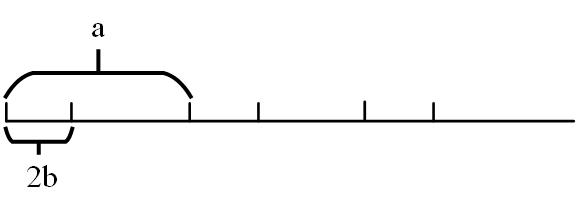
\includegraphics[width=8cm,height=3cm]{图3_1.jpg}        
    \caption{}                                                                                  
\end{figure}     
(1)若电子的势能函数可以表示为$\delta$函数之和
\begin{equation*}
    \begin{aligned}
        &W(x) = -V_0\sum_{n=0}^{N-1}[\delta(x-na+b)+\delta(x-na-b)]\\
    \end{aligned}
\end{equation*}
$V_0$为大于零的常数,请分别通过计算傅里叶系数得到第一、二布里渊区上的带隙宽度。\\
(2)在第(1)问的基础上,如果每个原子只有一个价电子,当$a>4b$时,晶体是否为导体?特殊地,当$a=4b$时,晶体是否为导体?请叙述理由。\\
(3)设$a>4b$,在第(1)问的基础上,如果每个原子有两个价电子,想要通过调控每个分子中两个原子的间距来使该一维晶体导电,请问$a$和$b$应该满足
怎样的关系?\\
\section*{4.(13分)室温$300K$时本征半导体$X$和$p$型掺杂半导体材料$Y$形成异质结,已知$X$和$Y$的禁带宽度分别为$E_{gX}=0.66eV$和$E_{gY}=1.42eV$,
电子亲和能分别为$\chi_X=4.13eV$和$\chi_Y=4.07eV$,本征载流子浓度分别为$n_{iX}=2.4\times10^{13}cm^{-3}$和$n_{iY}=1.79\times10^{6}cm^{-3}$,
Y的掺杂浓度为$N_a=10^{16}cm^{-3}$。}
(1)求导带能级差$\Delta E_C$和价带能级差$\Delta E_V$。\\
(2)求$X$和$Y$费米能级$E_{FX}$和$E_{FY}$的位置,以及它们之间的接触电势差$V_D$。\\
(3)画出平衡时该异质结的能带图,并在图中标注真空能级、费米能级、导带底和价带顶的位置,以及禁带宽度、电子亲和能、$\Delta E_C$、$\Delta E_V$、$V_D$。
(画出大致趋势即可,作图不要求数值比例严格)\\
\section*{5.(15分)有一长度为L的一价正负离子交错构成的一维晶格,平衡时正负离子间距为a,正负离子质量分别为2m和m,只计近邻两离子的相互作用势:
\begin{equation*}
    \begin{aligned}
        & U(r)=-\frac{q^2}{r}+\frac{b}{r^{2n}}\\
    \end{aligned}
\end{equation*}
其中,q为电子电荷,b和n为参量常数,求:}
(1)参数b(用q、n和a表示);\\
(2)已知简谐近似时,在平衡位置附近有$U(r)=U(a)+\frac{1}{2}\beta(r-a)^2$,求恢复力系数$\beta$。\\
(3)写出相邻的第2n和第2n+1两个离子的运动方程。考虑周期性边界条件,并分别代入简谐振动试解,根据方程解存在的条件,求出可能发生的格波频率解$\omega$。\\
(4)画出简约布里渊区中格波色散关系曲线示意图,标出驻波点。\\
(5)求长波极限时,光学波的频率$\omega_0$和声学波的频率$\omega_A$。\\


答案:\\
\section*{1.填空题}
(1)\ding{172}晶体\ding{173}晶格\ding{174}晶胞\ding{175}原胞\\
(2)\ding{172}面心立方\ding{173}共价\ding{174}复式\ding{175}体心立方\\
(3)\ding{172}能\ding{173}不能\\
(4)\ding{172}晶格的周期性势场\ding{173}负\ding{174}小于\\
(5)\ding{172}带隙中央\ding{173}导带\ding{174}价带\\
(6)\ding{172}$>$\ding{173}空穴\\
(7)\ding{172}导带底\ding{173}费米能级\\
(8)\ding{172}增大\ding{173}基本不变\ding{174}增大\\
(9)\ding{172}扩散\ding{173}空穴\ding{174}负\ding{175}空间电荷区\ding{176}从N区指向P区\ding{177}空间电荷区中间某位置\ding{178}反比
\ding{179}少数\ding{180}漂移\\
(10)\ding{172}P\ding{173}N\\
(11)\ding{172}>\ding{173}电子亲和能\\
(12)\ding{172}光学波\ding{173}低\ding{174}相邻原子位相相反,同种原子位相相同\ding{175}高\\
(13)\ding{172}$N$\ding{172}$2N$\\
(14)\ding{172}$P$\ding{173}$3.90625\times10^{21}m^{-3}$\\
\section*{2.}
(1)
\begin{equation*}
    \begin{aligned}
        & a = 0.142\sqrt3=0.2460nm\\
        & S = 6\times\frac{\sqrt3}{4}\times0.142^2=5.239\times10^{-2}nm^2\\
        & \bm{b_1} = \frac{2\pi}{\sqrt3a}(1,\sqrt3),\bm{b_2} = \frac{2\pi}{\sqrt3a}(1,-\sqrt3)\\
        & \lVert \bm{b_1} \rVert = \frac{4\pi}{\sqrt3a} = 29.50nm^{-1}, <\bm{b_1}, \bm{b_2}> = \frac{2\pi}{3}\\
    \end{aligned}
\end{equation*}
(2)
\begin{wrapfigure}{l}{4cm}                               
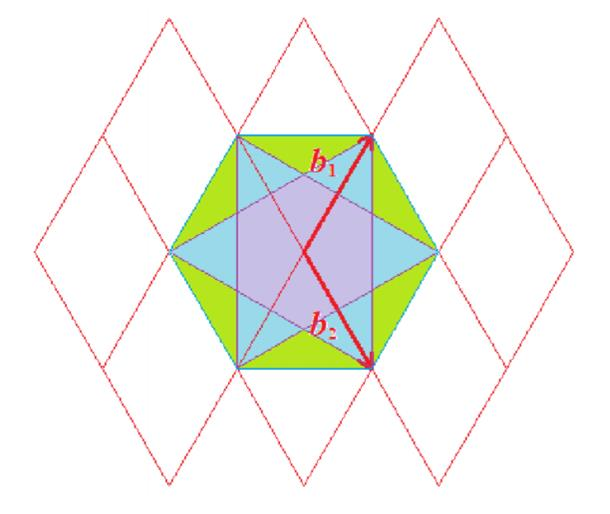
\includegraphics[width=4cm]{图3.jpg}                  
\caption*{}                                              
\end{wrapfigure}                                          
紫色、蓝色、绿色部分依次为第一、二、三布里渊区。\\
$S_1=S_2=S_3=(\frac{4\pi}{3a})^2\times\frac{\sqrt3}{4}\times6=753.6nm^{-2}$\\
(3)
$k_F = \sqrt{2\pi n} = 30.98nm^{-2}$\\
\section*{3.}
(1)
\begin{equation*}
    \begin{aligned}
        &W(x) = \sum V_n e^{j\frac{2\pi n}{a}x}, V_n = \frac{1}{a}\int_{-\frac{a}{2}}^{\frac{a}{2}}W(x)e^{-j\frac{2\pi n}{a}x}dx 
        =\frac{2V_0}{a}cos(\frac{2\pi nb}{a})\\
        &V_{g_1} = \lvert 2V_1\rvert = \frac{4V_0}{a}cos(\frac{2b}{a}\pi), 
        V_{g_2} = \lvert 2V_2\rvert = \frac{4V_0}{a}cos(\frac{4b}{a}\pi)\\
    \end{aligned}
\end{equation*}
(2)$a>4b$不是导体,$a=4b$是导体。\\
(3)$a=8b$\\
\section*{4.}
(1)\\
$\Delta E_C=\chi_X-\chi_Y = 0.06eV, \Delta E_V=\lvert(\chi_X+E_{gX})-(\chi_Y+E_{gY})\rvert = 0.7eV$\\
(2)
\begin{equation*}
    \begin{aligned}
        & E_{FX}=-(\chi_X+\frac{1}{2}E_{gX})=-4.46eV,E_{FiY}=-(\chi_Y+\frac{1}{2}E_{gY})=-4.78eV\\
        & E_{FY}=E_{FiY}-k_BTln(\frac{N_a}{n_i})=-5.36eV, V_D=\frac{E_{FX}-E_{FY}}{e}=0.9V\\
    \end{aligned}
\end{equation*}
(3)
\begin{figure}[H]                                        
    \centering                                                
    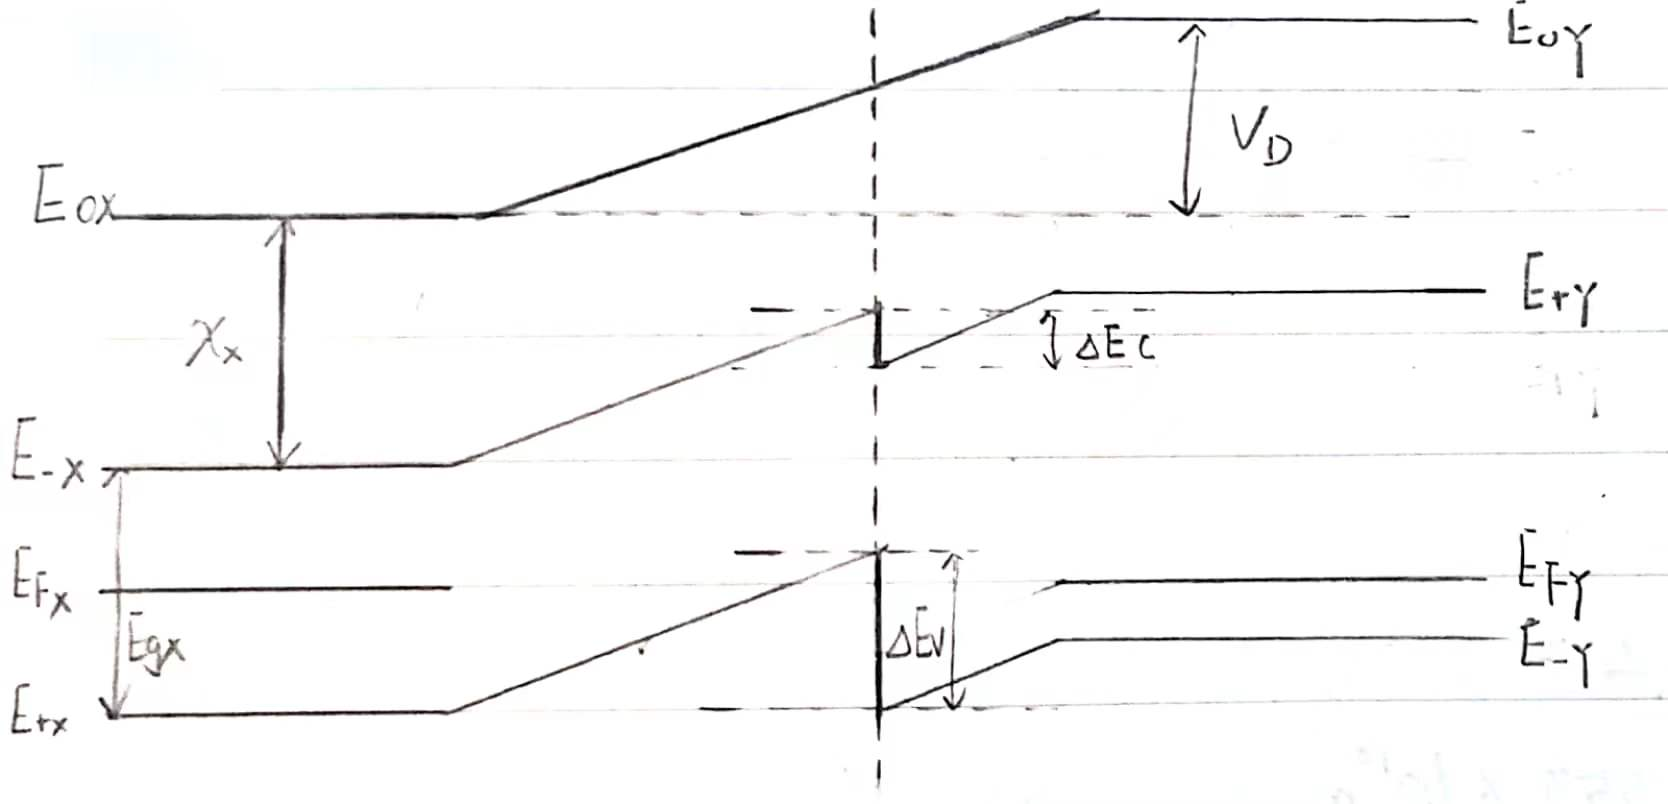
\includegraphics[width=8cm,height=4cm]{4-3.jpg}        
    \caption*{}                                                                                  
\end{figure}     
\section*{5.}
(1)
\begin{equation*}
    \begin{aligned}
       & \frac{dU}{dr}\bigg\lvert_a=\frac{q^2}{r^2}-\frac{2nb}{r^{2n+1}}=0, b=\frac{q^2}{2n}a^{2n-1}\\ 
    \end{aligned}
\end{equation*}
(2)
\begin{equation*}
    \begin{aligned}
        & U(r) = U(a)+\frac{dU}{dr}\bigg\lvert_a(r-a)+\frac{1}{2}\frac{d^2U}{dr^2}\bigg\lvert_a(r-a)^2 
        = U(a)+\frac{(2n-1)q^2}{2a^3}=U(a)+\frac{1}{2}\beta(r-a)^2\\
        & \beta = \frac{(2n-1)q^2}{a^3}\\
    \end{aligned}
\end{equation*}
(3)
\begin{equation*}
    \begin{aligned}
        & m\ddot\mu_{2n} = \beta(\mu_{2n+1}+\mu_{2n-1}-2\mu_{2n})\\
        & m\ddot\mu_{2n+1} = \beta(\mu_{2n+2}+\mu_{2n}-2\mu_{2n+1})\\
        & \mu_{2n} = Ae^{i(\omega t-2nka)}, \mu_{2n+1} = Be^{i(\omega t-(2n+1)ka)}\\
        & \Delta = (2\beta-m\omega^2)(2\beta-2m\omega^2)-4\beta^2sin(ka)cos(ka)=0\\
        & \omega^2 = \frac{\beta}{2m}(3+\sqrt{1+sin(2ka)})=\frac{(2n-1)q^2}{2ma^3}(3+\sqrt{1+sin(2ka)})\\
    \end{aligned}
\end{equation*}
(4)
\begin{figure}[H]                                        
    \centering                                                
    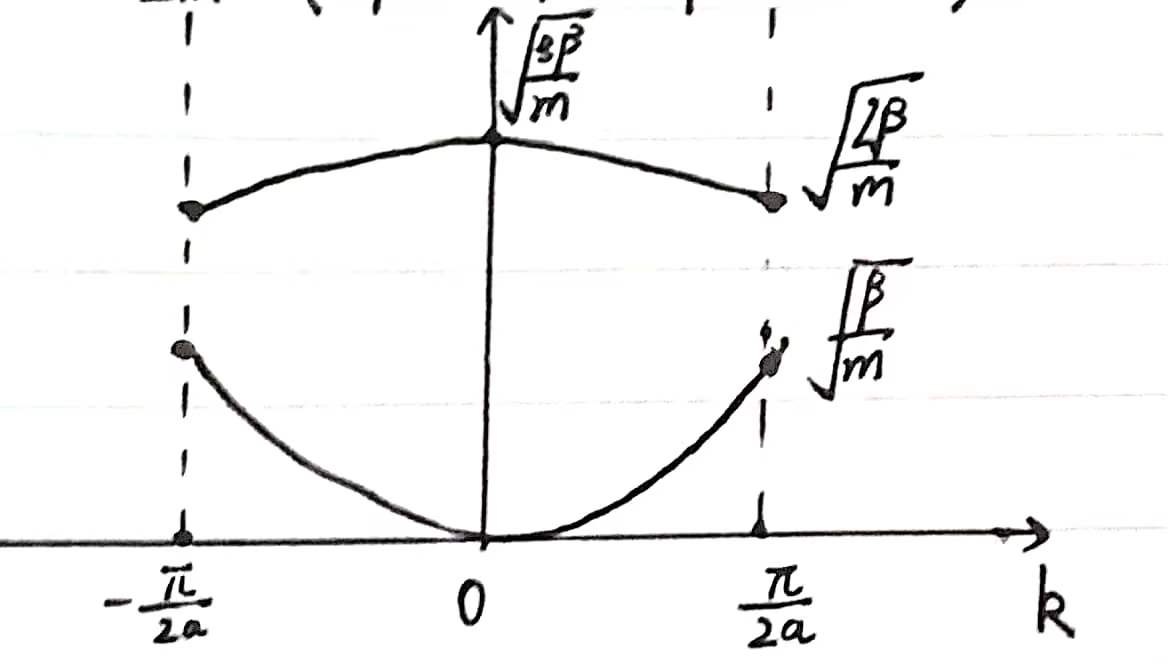
\includegraphics[width=6cm,height=4cm]{5-3.jpg}        
    \caption*{}                                                                                  
\end{figure}   
(5)
\begin{equation*}
    \begin{aligned}
        &\omega_A=0,\omega_0=\sqrt{\frac{3\beta}{m}}=\sqrt{\frac{3(2n-1)q^2}{ma^3}}\\
    \end{aligned}
\end{equation*}  
\end{document}



